\documentclass[aspectratio=169,11pt,svgnames,handout]{beamer}

\usepackage[czech]{babel}
\usepackage[czech=quotes]{csquotes}
\usepackage{graphicx}
\usepackage{enumitem}
\usepackage{amsmath}
\usepackage{mathtools}
\usepackage{float}
\usepackage{tikz}

% Flowchart stuff
\usetikzlibrary{shapes.geometric, arrows.meta, calc, positioning}
\tikzstyle{startstop} = [rectangle, rounded corners, minimum width=3cm, minimum
height=1cm,text centered, draw=black, fill=Red!30]
\tikzstyle{io} = [trapezium, trapezium left angle=70, trapezium right angle=110,
minimum width=3cm, minimum height=1cm, text centered, draw=black, fill=Blue!30]
\tikzstyle{process} = [rectangle, minimum width=3cm, minimum height=1cm, text
centered, draw=black, fill=Orange!30]
\tikzstyle{decision} = [diamond, aspect=2, minimum width=3cm, minimum height=.5cm, text
centered, draw=black, fill=Green!30]
\tikzstyle{connector} = [draw, -latex']

\usepackage{pgfopts}
\usepackage{xcolor}
\usepackage{tcolorbox}
\usepackage{booktabs}

\usetheme[
 titlestyle=style2,
 titleformat=smallcaps,
 sectionstyle=plain,
 slidestyle=cyber,
 headingcolor=theme,
 block=transparent
]{trigon}

\title{Externí paměť}
\subtitle{HDD, SSD, CD, Flash}
\date{\today}
\author{Adam Klepáč}
\institute[GEVO]{Gymnázium Evolution Jižní Město}
\biglogo[width=.2\textwidth]{logo}
\smalllogo[width=.1\textwidth]{logo}
\titlegraphic{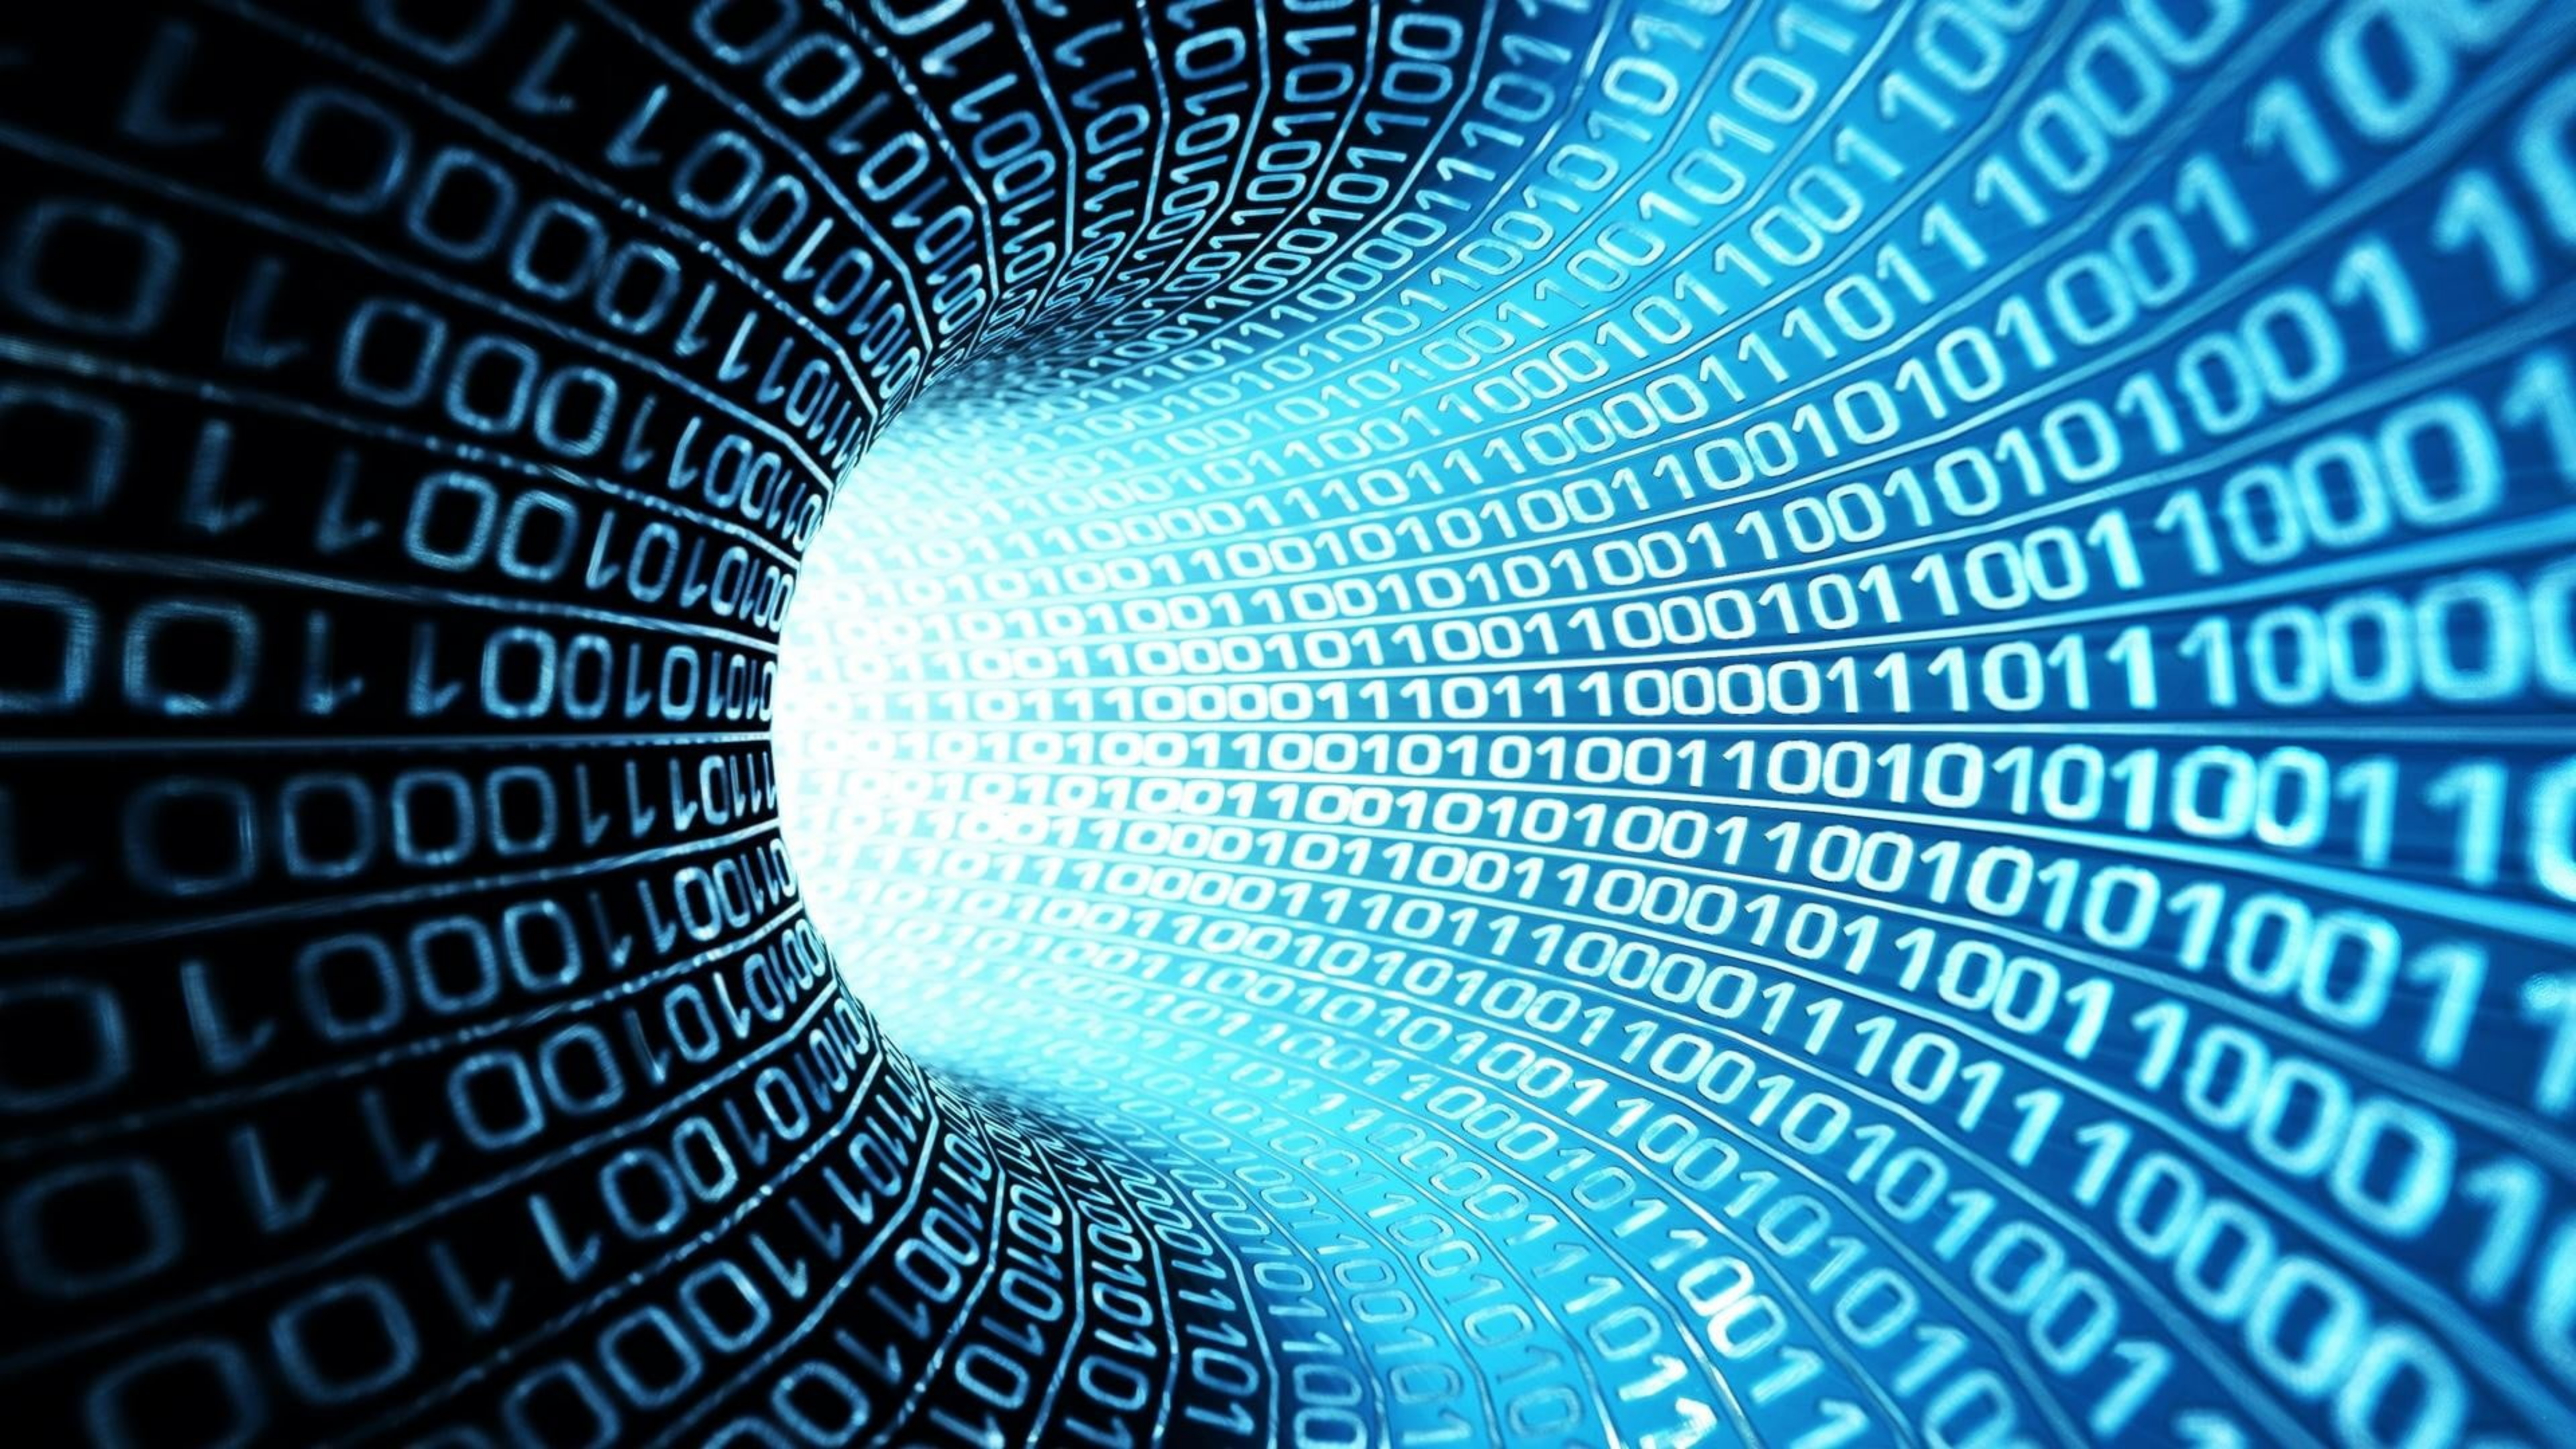
\includegraphics[height=\paperheight]{title.jpg}}

\def\subsectionname{}

% enumerate global settings
\setlist[enumerate,1]{label=\arabic*.}
\setlist[enumerate,2]{label=\alph*)}

% custom colors %
\definecolor{PCBlack}{HTML}{1B1B26}
\definecolor{PCBrown}{HTML}{642917}
\definecolor{PCGray}{HTML}{A6A7B5}
\definecolor{PCLavender}{HTML}{504456}
\definecolor{PCOrange}{HTML}{D16D1F}
\definecolor{PCBlue}{HTML}{2F4674}

\colorlet{tPrim}{PCBrown}
\colorlet{tSec}{PCLavender}
\colorlet{tAccent}{PCOrange}
\colorlet{tTheme}{PCBlue}
\colorlet{tTxt}{PCBlack}

\tcbset{
 boxsep=7pt,
 fonttitle=\sc,
 colframe=tGreyBg,
 colframe=tTheme,
 boxrule=1pt
}

\begin{document}
\titleframe

\begin{frame}
 \frametitle{Obsah}
 \tableofcontents
\end{frame}

\begin{frame}
 \frametitle{Externí paměť}
 \begin{tcolorbox}[title=Co je externí paměť]
  Externí pamětí myslíme jakékoli úložiště dat rozdílné od vnitřní paměti, tj.
  od CPU cache, RAM a VRAM (\textbf{V}ideo RAM -- vnitřní paměti GPU).
 \end{tcolorbox}
\end{frame}

\section{Typy externích pamětí}

\begin{frame}
 \frametitle{Typy externích pamětí}
 \textbf{Magnetická}
 \begin{itemize}[label=\textbullet]
  \item Floppy Disk, HDD
 \end{itemize}
 \pause
 \textbf{Optická}
 \begin{itemize}[label=\textbullet]
  \item CD, DVD, Blu-ray
 \end{itemize}
 \pause
 \textbf{Flash}
 \begin{itemize}[label=\textbullet]
  \item SD karta, USB disk, SSD
 \end{itemize}
\end{frame}

\section{Magnetická úložiště}

\begin{frame}
 \frametitle{Floppy Disk/Diskette}
 Úzký ohebný magnetický disk v čtvercovém plastovém uzávěru pokrytý tkaninou,
 která lapá prach během otáčení.\\
 \pause
 K přečtení je třeba vložit disketu do speciální mechaniky.
\end{frame}

\begin{frame}
 \frametitle{Floppy Disk/Diskette}
 \begin{center}
  \includegraphics[width=.5\textwidth]{floppy}
 \end{center}
\end{frame}

\begin{frame}
 \frametitle{HDD (\textbf{H}ard \textbf{D}isk \textbf{D}rive)}
 Skládá se z pohonu a vřetene, které točí kruhovou deskou (nebo více deskami)
 z~nemagnetického materiálu s~tenkým magnetickým povrchem.\\
 \pause
 Magnetický povrch zapisují a snímají pohyblivé hlavy, obvykle jedna na každou
 desku.
\end{frame}

\begin{frame}
 \frametitle{HDD -- čtení a zápis}
 Zapisování probíhá principem magnetické indukce:
 \begin{itemize}[label=\textbullet]
  \item Povrch desky je rozdělen na okruhy, které jsou pak rozděleny na sektory
   -- každý sektor obsahuje data (obvykle 4 KB) v podobně extrémně malých
   magnetizovaných oblastí.
  \pause
  \item Zapisování na disk probíhá vynucením konkrétního směru magnetického pole
   v~každé oblasti.
   \pause
  \item Hlava \textbf{nečte} orientaci každé oblasti, ale pouze rozdíl v
   magnetickém poli mezi dvěma sousedními oblastmi (protože je výrazně silnější).
  \pause
  \item Absence rozdílu značí $0$ a přítomnost $1$.
 \end{itemize}
\end{frame}

\begin{frame}
 \frametitle{HDD -- schéma komponent}
 \begin{center}
  \includegraphics[width=.5\textwidth]{hdd_big}
 \end{center}
\end{frame}

\begin{frame}
 \frametitle{HDD -- sektory}
 \begin{center}
  \includegraphics[width=.5\textwidth]{hdd_sector}
 \end{center}
\end{frame}

\begin{frame}
 \frametitle{HDD -- zápis a čtení}
 \begin{center}
  \includegraphics[width=.8\textwidth]{hdd_reading}
 \end{center}
\end{frame}

\section{Optická úložiště}

\begin{frame}
 \frametitle{CD, DVD, Blu-ray}
 CD (\textbf{C}ompact \textbf{D}isc), DVD (\textbf{D}igital \textbf{V}ersatile
 \textbf{D}isc) i Blu-ray pracují na témže principu, liší se pouze rychlostí
 čtení a velikostí.\\
 \pause
 Čtení z optických úložišť i zápis na ně je pomalejší než třeba na HDD.
 \pause
 Všechny tři typy disků mají tři varianty:
 \begin{itemize}[label=\textbullet]
  \item ROM (Read-Only Memory) -- z disků lze pouze číst;
  \item R (Recordable) -- disk je původně prázdný a lze na něj \textbf{jednou}
   zapsat data;
  \item RW (Re-Writable) -- na disk lze opakovaně zapisovat. Optická úložiště se
   ale velmi rychle ničí častým přepisem. Průměrný maximální počet přepisů je
   1000.
 \end{itemize}
\end{frame}

\begin{frame}
 \frametitle{Optická úložiště -- jak fungují}
 Optické disky mají jednu stranu tvořenou extrémně reflexivním materiálem.\\
 \pause
 Data jsou na této straně disku zapsána jako \uv{prohlubně} a čtena jsou
 laserem.\\
 \pause
 Když laser narazí na prohlubeň, světlo se neodrazí zpátky, což počítač
 interpretuje jako číslo $0$. Když se naopak laser odrazí od disku mimo
 prohlubeň, je tento signál interpretován jako $1$.\\
 \pause
 Kapacita disku záleží pouze na typu laseru, který je použit k jeho čtení. Čím
 menší jeho vlnová délka, tím blíž (a menší) u sebe prohlubně mohou být.\\
 \pause
 Když jsou data na disku přepsána, je třeba vždy strhnout celou jednu vrstvu
 materiálu, aby se nejdřív povrch vyrovnal, a pak znovu vyhloubit díry.
\end{frame}

\begin{frame}
 \frametitle{CD -- příklad čtení}
 \begin{center}
  \includegraphics[width=.8\textwidth]{cd_reading}
 \end{center}
\end{frame}

\end{document}
